\documentclass{article}

% FIXME: https://github.com/google-research/arxiv-latex-cleaner

% XXX: (mental anchor / looped / 3h) ->  UNDADASEA + LANE 8
%      https://www.youtube.com/watch?v=n_LcVqqHSY8
%      https://www.youtube.com/watch?v=vpeljtzB1a4

\usepackage{arxiv}

\usepackage[utf8]{inputenc} % allow utf-8 input
\usepackage[T1]{fontenc}    % use 8-bit T1 fonts
\usepackage{hyperref}       % hyperlinks
\usepackage{url}            % simple URL typesetting
\usepackage{booktabs}       % professional-quality tables
\usepackage{amsfonts}       % blackboard math symbols
\usepackage{nicefrac}       % compact symbols for 1/2, etc.
\usepackage{microtype}      % microtypography
\usepackage{lipsum}		% Can be removed after putting your text content
\usepackage{graphicx}
\usepackage{float}

%%% BONUS %%%
\usepackage[table]{xcolor}  % for colors (like `red`)
\usepackage[normalem]{ulem} % for underline
\usepackage{booktabs}       % for better table
\usepackage{bm}             % for special table cell (`cellcolor`)
\usepackage{hhline,soul}    % for `hl` command (highlight text)
\usepackage{amsmath}        % for multi-line math
\usepackage[bottom]{footmisc}% for footnotes
%%%%%%%%%%%%%

%%% BIBTEX %%%
% https://sunsite.icm.edu.pl/pub/CTAN/info/biblatex-cheatsheet/biblatex-cheatsheet.pdf
\usepackage[backend=bibtex, style=numeric, sorting=ynt]{biblatex}
\addbibresource{main.bib} %                       `ynt` vs. `ydnt`
\newcommand{\citep}[1]{\citeauthor*{#1} \cite{#1}} % for `fancy` cite style
%%%%%%%%%%%%%%

\newcommand{\ourjfasingle}{JFAStar}
\newcommand{\ourjfa}{Lord Vorotron} % okJFAuto / JFAstar
%\title{A survey of \emph{jump flooding algorithm} applied to Voronoi}
% \emph{\ourjfa}: Evolving Fast GPU Algorithm for
% Voronoi Diagram and Distance Transform in O(1) from JFA using AutoML
\title{lord vorotron: finding the best JFA variant for the coming winter} % $\approx$

\renewcommand{\headeright}{}
\renewcommand{\undertitle}{Draft}
\renewcommand{\shorttitle}{\ourjfa}

%\date{September 9, 1985}	% Here you can change the date presented in the paper title
%\date{} 					% Or removing it

\author{
  Maciej A.~Czyzewski\\
  Institute of Computing Science\\
  Poznan University of Technology\\
  Piotrowo 2, 60-965 Poznan, Poland\\
  \texttt{maciejanthonyczyzewski@gmail.com} \\
  \And
  Kamil~Piechowiak\\
  Institute of Computing Science\\
  Poznan University of Technology\\
  Piotrowo 2, 60-965 Poznan, Poland\\
  \texttt{kamil.cams@gmail.com} \\
}

\begin{document}

%%%%%%%%%%%%%%%%%%%%%%%%%%%%%%%%%%%%%%%%%%%%%%%%%%%%%%%%%%%%%%%%%%%%%%%%%%%%%%%%

\maketitle

\hl{\textbf{UWAGA!} Przenioslem fragmenty ze starego szkicu, teraz jednak czuje ze
powinnien byc to takie ogolne podsumowanie wszystkich mozliwych wariantow JFA - i
w jakich przypadkach sie sprawdzaja. A tak przyokazji nasza wersja z szumem+trikami
ktora dobrze dziala, no i dodatek taki ze mozna teraz zrobic sobie ensembla (a
nie jako glowny cel tej pracy). Dlatego wszystko co ponizej to praktycznie
random/bardzo mocny szkic. Wykresy to wizualizacja smaku.}
\newline

\begin{abstract}
This paper studies a practical usage of machine learning (AutoML) to automate
research towards discovering efficient Voronoi Diagram and Distance Transform
algorithms.  As the baseline we used the Jump Flooding Algorithm (JFA) - by
finding new mutations which works best for specific data, and then ensembling
them into one, we create new state-of-the-art algorithm in this field named
\textbf{\ourjfa} \hspace{0.01cm} with time complexity \textcolor{red}{$\approx$O(1)} and
work complexity \textcolor{red}{$\approx$O(N)}.
The algorithm is faster and produces more accurate approximations. It could be
extended into 3D space in a slice-by-slice manner.  We started from the
assumption that JFA has potential for improvement - some benefits can be
observed for specific data by adding random noise and adjusting the step size in
JFA.  This showed us that, AutoML could examine this space, and find the best
possible algorithm in each case.  In the further part of the work, we discuss
the results, compare the variants and ensemble for creating the final algorithm.
\end{abstract}

\hl{\textbf{CEL:} omawiamy dwa algorytmy? jeden nastepca JFA} -
\textbf{\ourjfasingle} \hspace{0.01cm} \hl{oraz ensembla po naszym score fn. -}
\textbf{\ourjfa}???????

\keywords{aaaaaaaaaaaaaaaaaa \and bbbbbbbbbbbbbbb \and ccccccccccccccccccc}

%%%%%%%%%%%%%%%%%%%%%%%%%%%%%%%%%%%%%%%%%%%%%%%%%%%%%%%%%%%%%%%%%%%%%%%%%%%%%%%%
\section{Introduction} %%%%%%%%%%%%%%%%%%%%%%%%%%%%%%%%%%%%%%%%%%%%%%%%%%%%%%%%%
%%%%%%%%%%%%%%%%%%%%%%%%%%%%%%%%%%%%%%%%%%%%%%%%%%%%%%%%%%%%%%%%%%%%%%%%%%%%%%%%

% FIXME: na wypadek zmiany tytulu w przyszlsoci!!!!!!!!!! ;-)
This paper\footnote{the original title for this paper was ``Lord Vorotron:
Finding the Best JFA Variant for the Coming Winter''} studies a practical usage of machine learning to automate research
towards discovering efficient Distance Transform algorithms (utilizing technique known as AutoML).
Thus, by finding mutations which works best for specific data, and then ensembling them into
one, we create new state-of-the-art algorithm in this field named \uline{\ourjfa \hspace{0.01cm} with
time complexity $\approx$O(1) and work complexity $\approx$O(N).}

Notable contribution to the quick algorithm that makes Distance Transform (DT)
using graphics hardware includes \citep{hoff1999fast} that creates a cone for
each input (point/seed) and renders those cones to obtain the Voronoi diagram as the lower envelope of these cones.
\cite{fischer2006fast} use planes tangent to a paraboloid and thus avoid the errors caused by the tessellation of the cones.
Unfortunately, the drawback of this approach is the significant amount of computation and the implementation complexity.

Jump flooding algorithm (JFA)\footnote{a novel pattern of
communication} is an interesting way to utilize the graphics processing unit to
efficiently compute Voronoi diagrams and distance transforms
\cite{rong2006jump}. This method is faster and produces more accurate results
\cite{rong2007variants}, and furthermore, it could be extended into 3D space in a slice-by-slice manner.
This is more effective than the previous research carried out by
\citep{sud2006interactive}, because the speed of JFA is almost independent to the number of seeds \cite{rong2007variants}.

Based on this research and findings, several efficient GPU-based algorithms which are either
work optimal or time optimal have been proposed including
SKW \cite{schneider2009gpu}, PBA \cite{cao2010parallel}, FastGPU \cite{de2017fast}, Honda's algorithm \cite{honda2017simple} and
WTO \cite{manduhu2019work}.

The main question that needs to be addressed now is whether JFA has potential
for improvement. We found some benefits for specific data by adding random noise
and adjusting the phase size in JFA. Therefore, this shows that, AutoML could examine this
unknown space, and find the best possible algorithm in each case.

For convenience, this work focus on the Voronoi diagram only - because this problem can be translated to DT \cite{rong2006jump}.
The algorithm would be an approximation of the output, thus we suggest using WTO
\cite{manduhu2019work} for exact DT (EDT). The major contributions of this paper are thus:

\begin{enumerate}
	\item Presenting new state-of-the-art variants of algorithm for Voronoi
		Diagram and Distance Transform: \newline
		\textbf{\ourjfasingle} - single best variant;
		\textbf{\ourjfa} - ensemble of weak variants; and
	\item Analyzing all possible variants of JFA: comparing error and speedup
		relative to bruteforce method
%\item Proposing, for an input set of seeds in a 2D grid, the first
%parallel algorithm in GPU to compute in constant time (i.e.
%independent of the number of seeds) a highly accurate
%Voronoi diagram and distance transform.
\end{enumerate}

%%%%%%%%%%%%%%%%%%%%%%%%%%%%%%%%%%%%%%%%%%%%%%%%%%%%%%%%%%%%%%%%%%%%%%%%%%%%%%%%
\section{Related Work} %%%%%%%%%%%%%%%%%%%%%%%%%%%%%%%%%%%%%%%%%%%%%%%%%%%%%%%%%
%%%%%%%%%%%%%%%%%%%%%%%%%%%%%%%%%%%%%%%%%%%%%%%%%%%%%%%%%%%%%%%%%%%%%%%%%%%%%%%%

Several efficient GPU-based algorithms which are either
work optimal or time optimal have been proposed including
JFA \cite{rong2006jump}, SKW \cite{schneider2009gpu},
PBA \cite{cao2010parallel}, FastGPU \cite{de2017fast}, Honda's algorithm \cite{honda2017simple} and
WTO \cite{manduhu2019work}.

\begin{table}[H] \centering
\begin{tabular}{@{}lllll@{}}
\toprule
Reference                & Algorithm    & Exactness   & Time         & Work         \\ \midrule
\citep{de2017fast}       & FastGPU      & Exact       & $O(n^3/p)$   & -            \\
\citep{cao2010parallel}  & PBA          & Exact       & $O(n)$       & $O(mN)$      \\
\citep{honda2017simple}  & based on SKW & Exact       & $O(n)$       & $O(N)$       \\
\citep{manduhu2019work}  & WTO          & \cellcolor{blue!25}\textbf{Exact}& \cellcolor{blue!25}$\bm{O(\log n)}$  & $O(N)$       \\
\citep{schneider2009gpu} & SKW          & Approximate & $O(n)$       & $O(N)$       \\
\citep{rong2006jump}     & JFA          & Approximate & $O(\log n)$  & $O(N\log n)$ \\ \bottomrule
In this paper            & \ourjfa      & \cellcolor{blue!25}\textbf{Approximate} & \cellcolor{blue!25}$\sim$$\bm{O(1)}$ & $\sim$$O(N)$ \\ \bottomrule
\end{tabular}
\vspace{1em}
\caption{Different GPU algorithms for computing EDT}
\end{table}

\subsection{Jump Flooding} %%%%%%%%%%%%%%%%%%%%%%%%%%%%%%%%%%%%%%%%%%%%%%%%%%%%%

\hl{redukcja i bridge pomiedzy intro (usunac subsection)}

co to jest jump flooding? tak naprawde to nie jest algorytm do voronoi-a tylko
pattern komunikacyjny w programowaniu rownoleglym - swojej pracy doktorskiej
autor tej techniki podaje wiele zastosowan jednak w swoich badaniach ogranicza
sie do Voronoi-a. glownym pytaniem roznych takich patternow jest ile potrzebnych
jest rund/operacji komunikacji aby zagwarantowac aby dana informacja zostanie
dostarczona. akurat w voronoi-u wiele komorek jest lokalna w skali calego
przykladu - wiec JFA ktora gwarantuje dostarczenie informacji globalnie do
kazdego punktu - wykonuje pewne niepotrzebne operacje.  szybkosc i zajetosc
pamieciowa JFA jest satysfakcujaca, jednak proste modyfikacje pokazuja ze
algorytm ten wykonuje sie szybciej w pewnych przypadkach (i to typowych).
dlatego naturalnym pytanie powinno byc w jakich oraz jakie modyfikacje wplywaja
na szybkosc dzialania.

\subsection{AutoML} %%%%%%%%%%%%%%%%%%%%%%%%%%%%%%%%%%%%%%%%%%%%%%%%%%%%%%%

\hl{przeniesc do Proposed Method}

okay przenioslem - dodac prace co tez tak szuka algosow

%%%%%%%%%%%%%%%%%%%%%%%%%%%%%%%%%%%%%%%%%%%%%%%%%%%%%%%%%%%%%%%%%%%%%%%%%%%%%%%%
\section{Proposed Method} %%%%%%%%%%%%%%%%%%%%%%%%%%%%%%%%%%%%%%%%%%%%%%%%%%%%%%
%%%%%%%%%%%%%%%%%%%%%%%%%%%%%%%%%%%%%%%%%%%%%%%%%%%%%%%%%%%%%%%%%%%%%%%%%%%%%%%%

\hl{przepisac ten szkic bo jezyk sie placzy}

JFA opiera sie na tym ze infomacja jest przekazywana ??????.  Przekazanie odbywa
sie w log(n) krokach. Wiec przeprowadzilismy krotki eksperyment applyujac losowy
szum na wejsciowa masce. Okazalosie sie ze ilosc potrzebnych krokow spadla -
powstaly losowe shortcuty.  Co oznacza ze powinny istniec inne "mutacje"
algorytmow lepsze w pewnych okreslonych przypadkach.  Wiec szukanie najszybszego
algorytmu bedzie nastepujace:

\begin{itemize}
\item Wymyslenie wszystkich mozliwych wariantow JFA
\item Mutacje i zapisanie najlepszych wersji dla danej domeny
\item Ensemblacja algorytmow tak aby wybierac najlepszy variant dla danej domeny
\end{itemize}

\subsection{Domain Space} %%%%%%%%%%%%%%%%%%%%%%%%%%%%%%%%%%%%%%%%%%%%%%%%%%%%%%

jakie domeny i dlaczego (i jak dzialaly gen\_uniform, \hl{gen\_polar, gen\_grid})

\begin{itemize}
	\item \textbf{shapes}: \{(64, 64), (128, 128), (256, 256), (512, 512), (768,
		768)\}
	\item \textbf{cases}:
        \begin{itemize}
			\item gen\_uniform: seeds=1,
			\item gen\_uniform: seeds=2,
			\item gen\_uniform: density=0.0001,
			\item gen\_uniform: density=0.001,
			\item gen\_uniform: density=0.01,
			\item gen\_uniform: density=0.02,
			\item gen\_uniform: density=0.03,
			\item gen\_uniform: density=0.04,
			\item gen\_uniform: density=0.05,
			\item gen\_uniform: density=0.1,
		\end{itemize}
\end{itemize}

\subsection{Search Space} %%%%%%%%%%%%%%%%%%%%%%%%%%%%%%%%%%%%%%%%%%%%%%%%%%%%%%

\hl{bridge z score function gdziekolwiek to bedzie}
\hl{obliczyc ile jest aktulanie wersji algosow np. czy jest to juz 2do14 jak
mamy 3xreal w wielomianie AKTUALNIE JEST okolo 7,200?}

jakie modyfikacje, na to osobna sekcja? wiec co tu napisac
chyba tylko o zlozonosci problemu i ze kod jest skladany i testowany a niektore
wersje sa pomijane zgodnie z dzialaniem gp\_minimize (Bayesian optimization
using Gaussian Processes).

w naszym wypadku zdefiniowalismy pewien zbior variantow pewnych czesci
algorytmu (Search Space), modul testujacy dana mutacje/wariant - sklada kod kernela a pozniej go weryfikuje na naszej Domain Space.

\subsection{Score Function} %%%%%%%%%%%%%%%%%%%%%%%%%%%%%%%%%%%%%%%%%%%%%%%%%%%

\hl{SCORE CZY METRIC?}
\hl{roznica w pikselach pomiedzy bruteforce a algorytmem - napisac o tym / tez
ze to wszystko to ilorazy do bruteforce}

dla voronoi-a interesuja nas 2 parametry Error oraz Szybkosc, aby wyniki byly
wiarygodne porownujemy je z bruteforcem (a wiec bedzie to iloraz).
aby ocenic dana mutacje musimy przypisac jakis Score danej wersji, wiec uzylismy
wzor ponizej

\begin{align}
S(x,y) = max\{0, x \cdot (100-y^{1.5})\}, \\
0 \leq y \leq 100, 0 < x
\end{align}

ktory kaze za zbyt wysokie errory, dajac zerowy wynik - skladnik przy y rosnie
szybciej niz x wiec gdy przekroczy 100 da nam ujemny wynik - czyli 0.

\subsection{Optimizer} %%%%%%%%%%%%%%%%%%%%%%%%%%%%%%%%%%%%%%%%%%%%%%%%%%%%%%%%%

\hl{opisac dwie osobne taktyki optymalizacji dla best single vs. ensemble}

mozemy napisac ze korzystalismy z forest/gp minimize, ale tez wspomniec ze aby
miec najlepszy best single to trzeba bylo optymalizowac rownoczesnie cala
przestrzen (od malych do duzych, gestych po rzadkie), a zeby miec najlepszego
Vorotrona - czyli ensembla to trzeba bylo dla kazdej domeny z optymalizowac a
pozniej jedynie zrobic balancera!!!!!!!!!!!!

\subsection{Ensemble} %%%%%%%%%%%%%%%%%%%%%%%%%%%%%%%%%%%%%%%%%%%%%%%%%%%%%%%%%%

patrzac na rezultaty mozemy znalesc jaki algorytm najlepiej sprawdza sie w
zadanej domenie. np. widac ze dla malej ilosci seedow (malo gestych przypadkow,
ktore maja mala powierzchnie) oplaca sie uzyc bruteforce. Dla kolejnych
wiekszych przypadkow innych wariantow JFA. Jak wybrac algorytm? Kazdy przypadek ma `shape` oraz `num` wiec mozna na CPU wysemplowac
pare punktow albo odrazu obliczyc gestosc i wybrac odpowiedni algorytm.
To takich ensemblacji najlepiej sprawdzi sie drzewo decyzyjne (moze byc boostowane).

%%%%%%%%%%%%%%%%%%%%%%%%%%%%%%%%%%%%%%%%%%%%%%%%%%%%%%%%%%%%%%%%%%%%%%%%%%%%%%%%
\section{Variants} %%%%%%%%%%%%%%%%%%%%%%%%%%%%%%%%%%%%%%%%%%%%%%%%%%%%%%%%%%%%%
%%%%%%%%%%%%%%%%%%%%%%%%%%%%%%%%%%%%%%%%%%%%%%%%%%%%%%%%%%%%%%%%%%%%%%%%%%%%%%%%

\hl{ZROBIC LADNE RYSUNECZKI w Google Slides - eksport to pdf!}
wyjasnic slownictwo? np. co okreslamy przez anchor
i wyjasnic jak powstaly nazwy? np. Circle11Dual|Factor3+Noise

\subsection{Noise} %%%%%%%%%%%%%%%%%%%%%%%%%%%%%%%%%%%%%%%%%%%%%%%%%%%%%%%%%%%%%

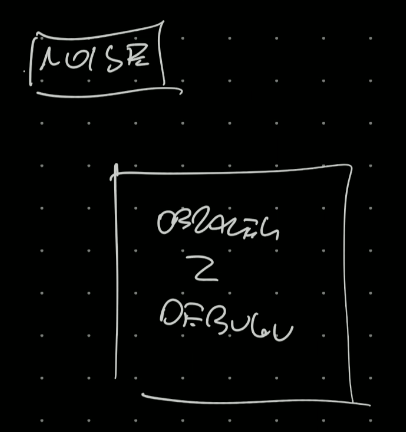
\includegraphics[width=0.5\linewidth]{../figures/idea_noise}

\hl{w poczatkowej wersji dodanie szumu pozwolilo zmienic zlozonosc - dodatkowo
mamy na to dowod kamila}

przed wykonaniem algorytmu punkty informacja o punktach jest losowo rozrzucana
po macierzy - tworzac przypadkowe short-cuty

\subsubsection{Local Noise} %%%%%%%%%%%%%%%%%%%%%%%%%%%%%%%%%%%%%%%%%%%%%%%%%%%%%%%

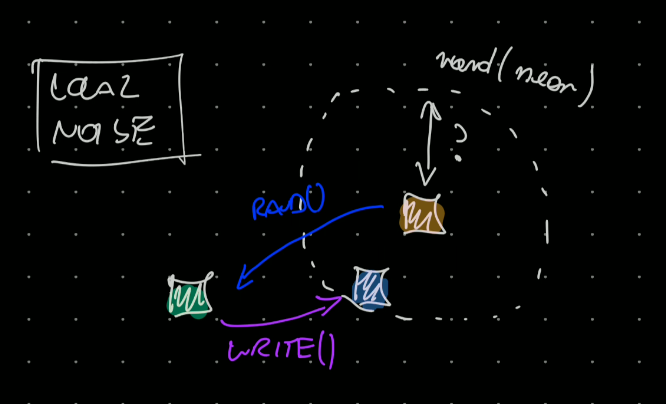
\includegraphics[width=0.5\linewidth]{../figures/idea_local_noise}

\hl{czy jest mozliwe losowanie szumu w takich plamach? aby lokalne seedy
losowaly lokalne seedy? - albo probuja modyfikowac wylosowany - hehe - czyli
prostujac jestem na pozycji (x,y) wylosowalem punkt (a,b) rzucam nim w okolice
(a+rand(density), b+rand(density)}

\subsection{Anchor Type} %%%%%%%%%%%%%%%%%%%%%%%%%%%%%%%%%%%%%%%%%%%%%%%%%%%%%%%

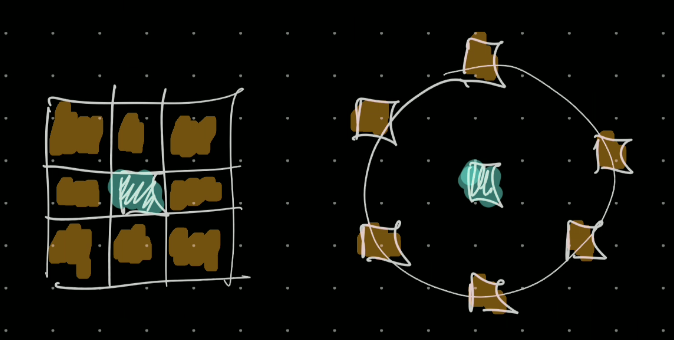
\includegraphics[width=0.5\linewidth]{../figures/idea_anchor_type}

orginalnalnie jest to kwadrat 3x3, my proponujemy okrag (rownomierny), lub
\hl{losowane punkty na okregu (doimplementowac)}.

\subsubsection{Anchor Num} %%%%%%%%%%%%%%%%%%%%%%%%%%%%%%%%%%%%%%%%%%%%%%%%%%%%%%%%

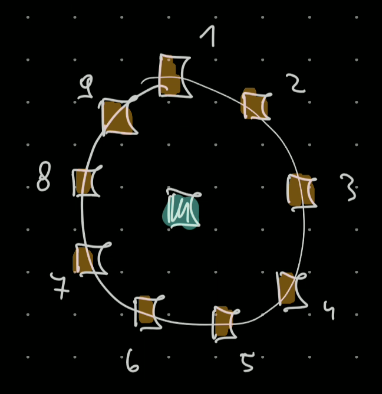
\includegraphics[width=0.5\linewidth]{../figures/idea_anchor_num}

tylko dla okregow?
ile ma byc punktow w anchorze (np. na okregu).
\hl{czy da sie to sensownie zaimplementowac dla kwadratu? tak naprawde tylko
3x3, 5x5 maja jakikolwiek sens}

\subsection{Anchor Double} %%%%%%%%%%%%%%%%%%%%%%%%%%%%%%%%%%%%%%%%%%%%%%%%%%%%%

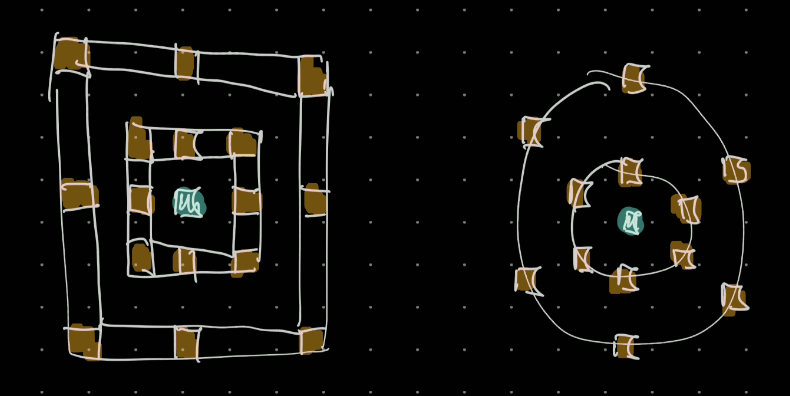
\includegraphics[width=0.5\linewidth]{../figures/idea_anchor_double}

oprocz pojedynczego anchora, mozliwe jest uzycie podwojnej warstwy anchorow
(czyli np. male kolko i wieksze) - idea - male kolko jest dokladne - a wielkie
jest skautujace (w sumie to podobny mechanizm jak w Lookahead - wolny/szybki)

\subsubsection{Anchor Distance Ratio}

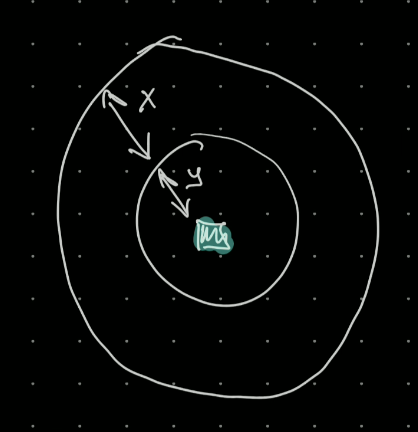
\includegraphics[width=0.5\linewidth]{../figures/idea_anchor_distance_ratio}

\hl{ratio pomiedzy zewnetrznymi a wewnetrznymi (doimplementowac) - mozliwosc od
0 do 1}

\subsubsection{Anchor Number Ratio}

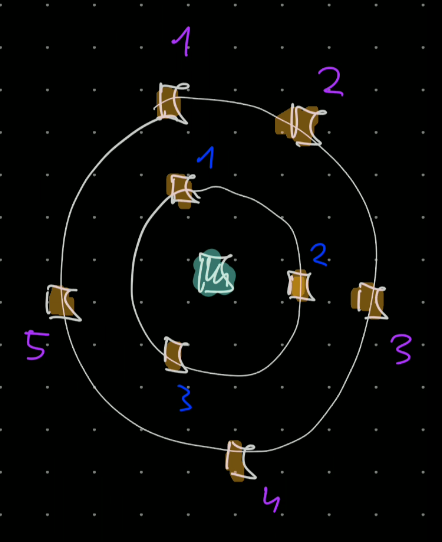
\includegraphics[width=0.5\linewidth]{../figures/idea_anchor_number_ratio}

\hl{ratio ale ilosciowe pomiedzy zewnetrznymi a wewnetrznymi (doimplementowac) -
czyli np. 5 na zewnetrznym a na bliskim 10}

\subsection{Step Function} %%%%%%%%%%%%%%%%%%%%%%%%%%%%%%%%%%%%%%%%%%%%%%%%%%%%%

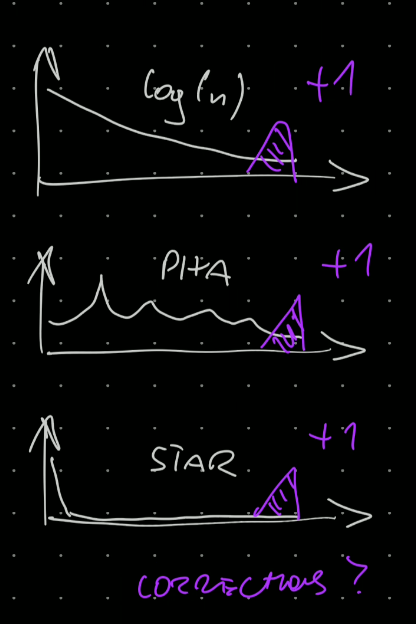
\includegraphics[width=0.5\linewidth]{../figures/idea_step_function}

aktualnie 3 warianty, standart JFA, zmieniona podstawa na 3, oraz logstar krokow,
powinna istniec tez wersja 4-ta, uzalezniona od num oraz shape - pozwalajaca na
robienie \hl{piloksztaltnych lub isogaussowaskich ciagow}.

\hl{wielomian z 3 parametrami (uzalezniony od dwoch
wejsci - shape, num)}

\subsubsection{Correction???} %%%%%%%%%%%%%%%%%%%%%%%%%%%%%%%%%%%%%%%%%%%%%%%%%%%%%%%%

mozna domimplementowac flage dla +1, +2 (jak u JFA), lub przechowywanie 2
najlepszych i ich przekazywanie (pewnie duzo wolniejsze wiec sie nie oplaca)

%%%%%%%%%%%%%%%%%%%%%%%%%%%%%%%%%%%%%%%%%%%%%%%%%%%%%%%%%%%%%%%%%%%%%%%%%%%%%%%%
\section{Results} %%%%%%%%%%%%%%%%%%%%%%%%%%%%%%%%%%%%%%%%%%%%%%%%%%%%%%%%%%%%%%
%%%%%%%%%%%%%%%%%%%%%%%%%%%%%%%%%%%%%%%%%%%%%%%%%%%%%%%%%%%%%%%%%%%%%%%%%%%%%%%%

\hl {przeniesc legende? JAKO OSOBNY PDF? i podac w tej sekcji - tak sie nie robi
ale bylo by ok i czytelnie + wiecej miejsca na wykresy a przypadkow bedzie
wiecej}

\subsection{Performance} %%%%%%%%%%%%%%%%%%%%%%%%%%%%%%%%%%%%%%%%%%%%%%%%%%%%%%%

wykres zostal zrobiony poprzez posortowanie scorow - dzieki temu widac roznice w
przyroscie i latwo dostrzec ktory algorytm ma najwyzszy score lub jaka ma
chaktersytyke (np. jest bardzo skuteczny dla waskiej grupy przykladow)

\begin{figure}[H]
	\centering
	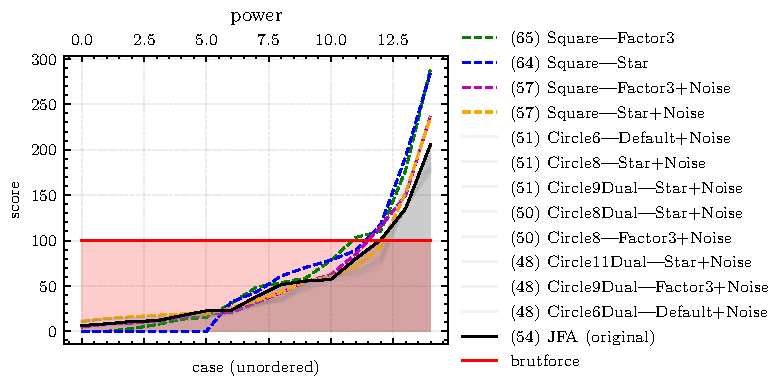
\includegraphics[width=\linewidth]{../figures/figure-4-power}
	\caption{bla bla bla}
	\label{fig:abstract}
\end{figure}

\subsection{Performance? ale taki inny} %%%%%%%%%%%%%%%%%%%%%%%%%%%%%%%%%%%%%%%%

te same dane jak w poprzedniej sekcji tylko nie posortowane - dlatego widac jak
wygladaja "gorki" dla danych shapow i rosnacych gestosci

\begin{figure}[H]
	\centering
	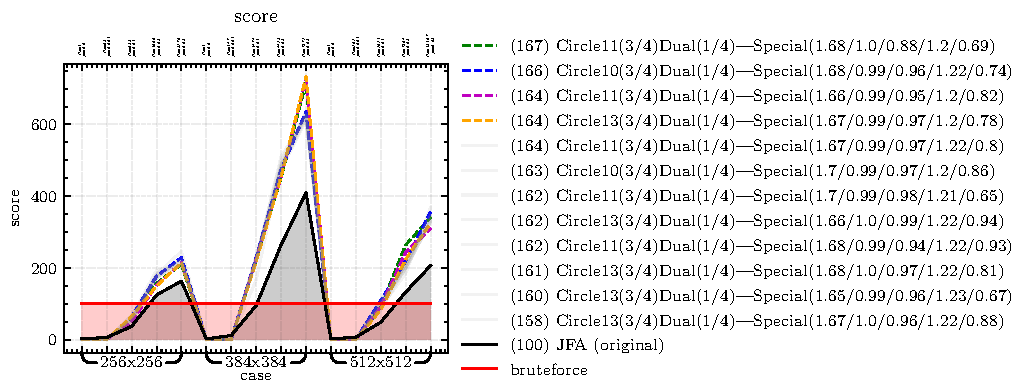
\includegraphics[width=\linewidth]{../figures/figure-3-score}
	\caption{bla bla bla}
	\label{fig:abstract}
\end{figure}

\begin{table}[H]
	\centering
	\begin{tabular}{lrrrllr}
\hline
 Algorithm                  &   $\rho$=0.0003 &   $\rho$=0.001 &   $\rho$=0.0099 & $\rho$=0.0298   & $\rho$=0.0499   &   Avg. score \\
\hline
 Square|Factor3             &             0   &           13.2 &            55.5 & \textbf{122.0}  & \textbf{169.3}  &           71 \\
 Square|Star                &             0   &            0   &            41.7 & \textbf{115.2}  & \textbf{161.5}  &           63 \\
 Square|Star+Noise          &            12.3 &           19   &            48.4 & 96.3            & \textbf{142.3}  &           63 \\
 Square|Factor3+Noise       &             7.9 &           13.6 &            43.5 & 91.6            & \textbf{145.2}  &           60 \\
 Circle8Dual|Default        &             0   &            9.8 &            39.3 & 85.6            & \textbf{123.3}  &           51 \\
 Circle10|Star+Noise        &            11.8 &           16.3 &            43.4 & 79.2            & 98.7            &           49 \\
 Circle10Dual|Factor3+Noise &             5.5 &           10.9 &            37.8 & 81.4            & \textbf{110.6}  &           49 \\
 Circle8Dual|Factor3+Noise  &             6.8 &           12.7 &            42.2 & 82.7            & 94.2            &           47 \\
 Circle10Dual|Star          &             0   &            0   &            28.2 & 85.0            & \textbf{124.2}  &           47 \\
 Circle11Dual|Factor3+Noise &             6   &           12   &            35.2 & 76.9            & \textbf{107.2}  &           47 \\
 Circle10Dual|Factor3       &             0   &            4.8 &            40.8 & 80.2            & \textbf{109.3}  &           47 \\
 Circle12|Star+Noise        &            10.6 &           14.7 &            37   & 70.3            & 87.2            &           43 \\
 Circle13|Factor3+Noise     &             6.2 &           10.4 &            32.6 & 70.9            & 92.2            &           42 \\
 Circle15Dual|Star          &             0   &            1.6 &            35.8 & 68.2            & \textbf{101.9}  &           41 \\
 Circle17Dual|Star          &             0   &            1.3 &            34.4 & 65.0            & 95.4            &           39 \\
 Circle6|Factor3+Noise      &             7.7 &           15.7 &            53.2 & 79.6            & 34.9            &           38 \\
 Circle7Dual|Default        &             0   &            6.4 &            37   & 66.7            & 79.7            &           37 \\
 Circle6Dual|Default        &             0   &            4.8 &            36.2 & 67.2            & 79.0            &           37 \\
 Circle6Dual|Star+Noise     &            14.7 &           20.9 &            42.1 & 59.2            & 32.4            &           33 \\
 Circle8Dual|Star           &             0   &            0   &             0   & 49.0            & 78.7            &           25 \\
 Circle9Dual|Star           &             0   &            0   &             0.2 & 39.1            & 74.9            &           22 \\
 Circle9Dual|Factor3        &             0   &            0   &             5.4 & 35.9            & 69.9            &           22 \\
 SquareDual|Factor3         &             0   &            4.9 &            19.2 & 35.8            & 49.8            &           21 \\
 Circle8Dual|Factor3        &             0   &            0   &             5.8 & 37.6            & 64.2            &           21 \\
 Circle10|Factor3           &             0   &            1.1 &            12.9 & 32.5            & 52.6            &           19 \\
 Circle14|Factor3           &             0   &            1   &            10.7 & 36.4            & 50.1            &           19 \\
 Circle9|Factor3            &             0   &            1.1 &             9.5 & 31.6            & 46.0            &           17 \\
 Circle10|Star              &             0   &            0   &             2.8 & 30.9            & 49.0            &           16 \\
 SquareDual|Default+Noise   &             2.1 &            3.5 &            12.3 & 26.7            & 37.8            &           16 \\
 Circle7Dual|Factor3        &             0   &            0   &             0   & 2.5             & 0.0             &            0 \\
 Circle7Dual|Star           &             0   &            0   &             0   & 1.9             & 0.0             &            0 \\
 Circle6Dual|Star           &             0   &            0   &             0   & 0.0             & 0.1             &            0 \\
\hline
\end{tabular}
	\newline
	\caption{domain: 32x32, 64x64, 128x128, 256x256}
\end{table}

\subsection{Error Rate} %%%%%%%%%%%%%%%%%%%%%%%%%%%%%%%%%%%%%%%%%%%%%%%%%%%%%%%%

score jest scisle powiazany z errorem ale tutaj przejrzyscie widac w jakich
przypadkach jest naprawde zle i ile (szarych) czesto jest bardzo szybkich - ale
rowniez bardzo blednych dlatego maja finalnie niskie scory

\begin{figure}[H]
	\centering
	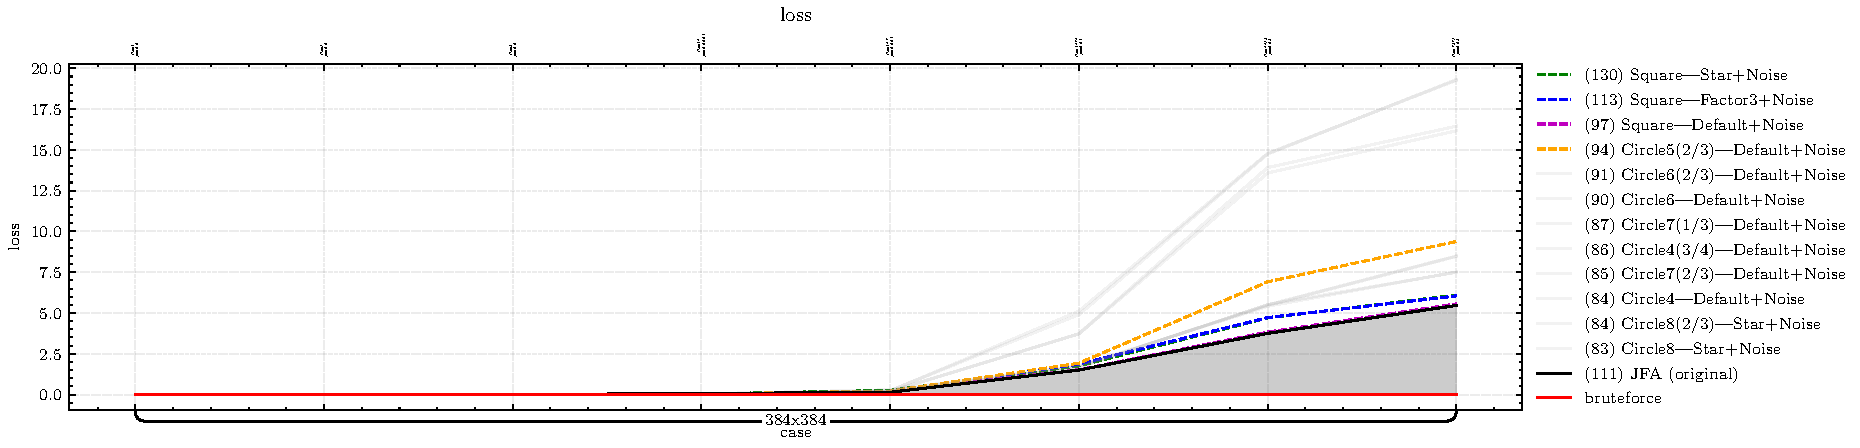
\includegraphics[width=\linewidth]{../figures/figure-2-loss}
	\caption{bla bla bla}
	\label{fig:abstract}
\end{figure}

\subsection{Objectives} %%%%%%%%%%%%%%%%%%%%%%%%%%%%%%%%%%%%%%%%%%%%%%%%%%%%%%%%

\hl{naprawic generowanie tego wykresu}

czyli co ma wplyw na co (w sumie to najwazniejsze mialo byc w pracy)

\begin{figure}[H]
	\centering
	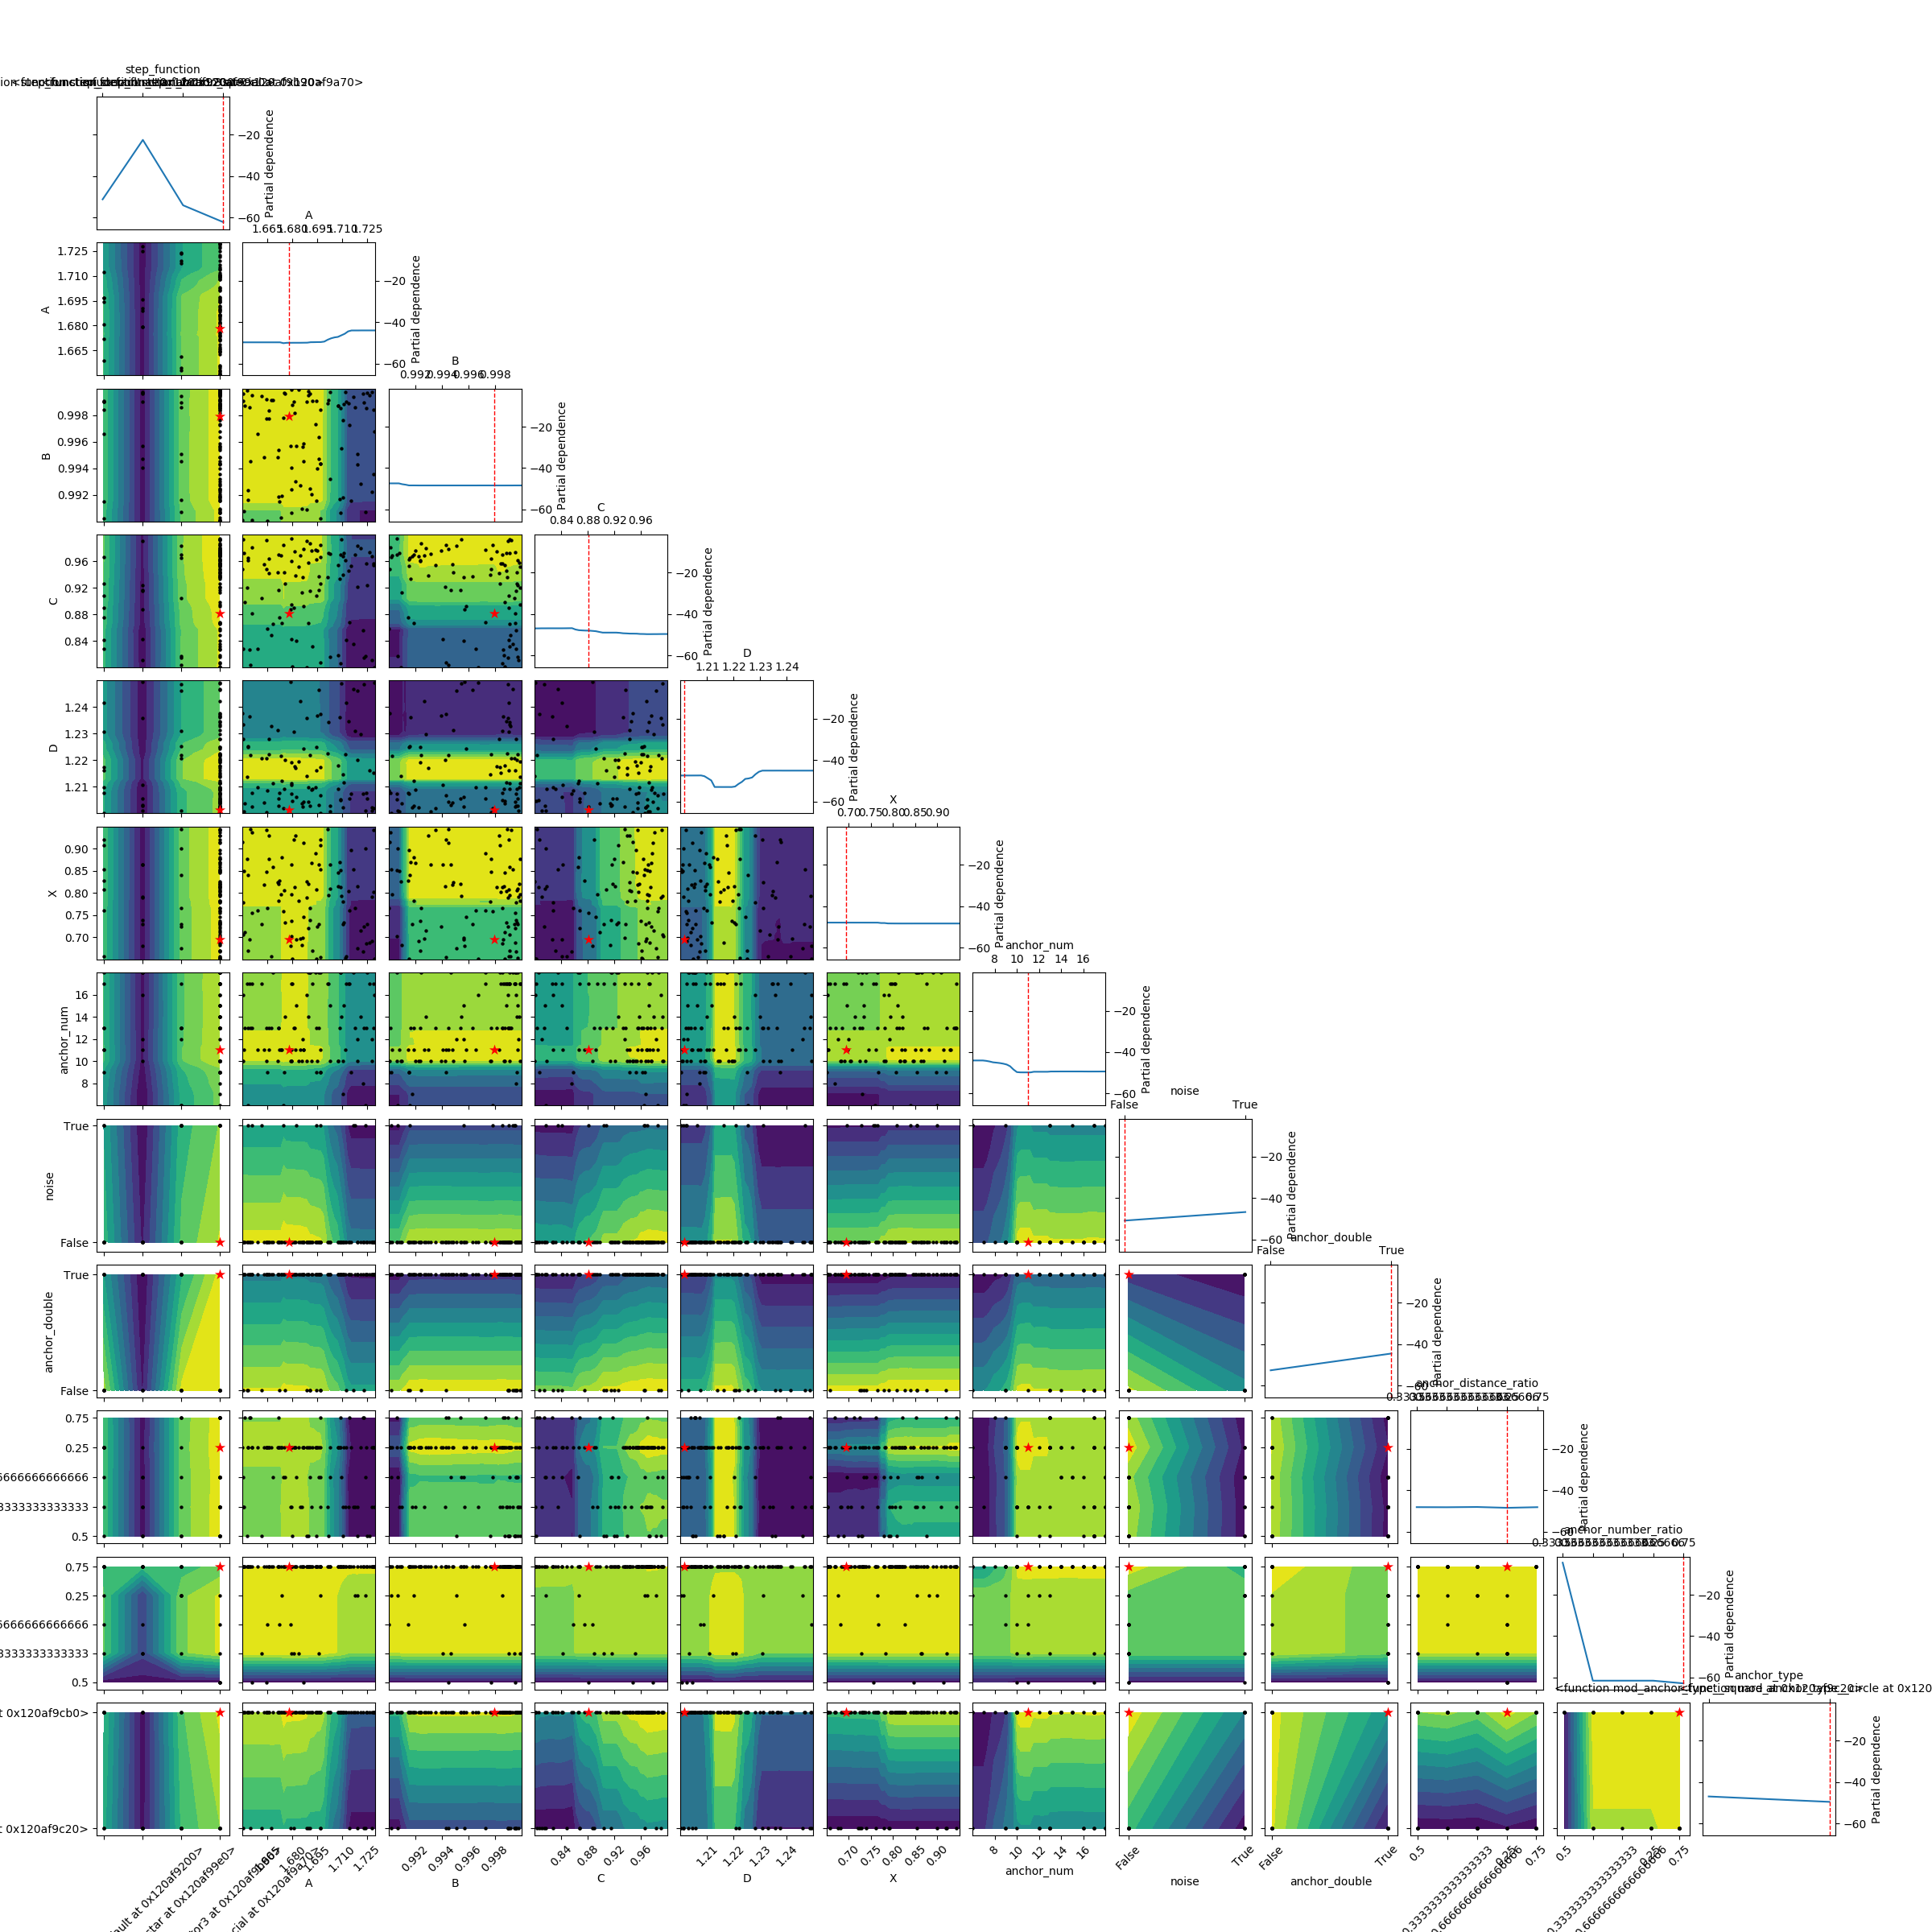
\includegraphics[width=\linewidth]{../figures/raport}
	\caption{bla bla bla}
	\label{fig:abstract}
\end{figure}

%%%%%%%%%%%%%%%%%%%%%%%%%%%%%%%%%%%%%%%%%%%%%%%%%%%%%%%%%%%%%%%%%%%%%%%%%%%%%%%%
\section{Practical Usage} %%%%%%%%%%%%%%%%%%%%%%%%%%%%%%%%%%%%%%%%%%%%%%%%%%%%%%
%%%%%%%%%%%%%%%%%%%%%%%%%%%%%%%%%%%%%%%%%%%%%%%%%%%%%%%%%%%%%%%%%%%%%%%%%%%%%%%%

\hl{polaczyc z Conclusions}

Jest wiele projektow ktore potrzebuje DT lub voronoi-a. Jedyne dwa praktyczne
przyklady z tej pracy to SOTA dla JFA - czyli JFAstar, oraz praktyczny Ensemble
(uwzgledniajacy np. bruteforce dla malych instancji).

%%%%%%%%%%%%%%%%%%%%%%%%%%%%%%%%%%%%%%%%%%%%%%%%%%%%%%%%%%%%%%%%%%%%%%%%%%%%%%%%
\section{Conclusions} %%%%%%%%%%%%%%%%%%%%%%%%%%%%%%%%%%%%%%%%%%%%%%%%%%%%%%%%%%
%%%%%%%%%%%%%%%%%%%%%%%%%%%%%%%%%%%%%%%%%%%%%%%%%%%%%%%%%%%%%%%%%%%%%%%%%%%%%%%%

This paper presents the GPU's effective, almost constant, algorithm for calculating the Euclidean distance transform (DT) approximation for 2D and higher dimensional images.
%
As mentioned in \cite{cao2010parallel}, it remains challenging to balance the workload in such an approach.
%
\textit{\ourjfa} does not explicitly solve this issue but, by constructing an alternative solution utilizing random shortcuts and parameter estimation, it makes it a reasonable approximation.
%
In practice, such a constant time algorithm is useful in many interactive applications, such as tessellations, rendering, and image processing, involving \cite{rong2006jump}.

%%%%%%%%%%%%%%%%%%%%%%%%%%%%%%%%%%%%%%%%%%%%%%%%%%%%%%%%%%%%%%%%%%%%%%%%%%%%%%%%
\section{Acknowledgements} %%%%%%%%%%%%%%%%%%%%%%%%%%%%%%%%%%%%%%%%%%%%%%%%%%%%%
%%%%%%%%%%%%%%%%%%%%%%%%%%%%%%%%%%%%%%%%%%%%%%%%%%%%%%%%%%%%%%%%%%%%%%%%%%%%%%%%

\hl{Dziekuje swojemu psu!Dziekuje swojemu psu! Dziekuje swojemu psu! Dziekuje swojemu psu! Dziekuje swojemu psu! Dziekuje swojemu psu! Dziekuje swojemu psu! Dziekuje swojemu psu! Dziekuje swojemu psu! Dziekuje swojemu psu! Dziekuje swojemu psu! Dziekuje swojemu psu! Dziekuje swojemu psu! Dziekuje swojemu psu! Dziekuje swojemu psu! Dziekuje swojemu psu! Dziekuje swojemu psu! Dziekuje swojemu psu! Dziekuje swojemu psu! Dziekuje swojemu psu! Dziekuje swojemu psu! Dziekuje swojemu psu! Dziekuje swojemu psu! Dziekuje swojemu psu!  }

%%%%%%%%%%%%%%%%%%%%%%%%%%%%%%%%%%%%%%%%%%%%%%%%%%%%%%%%%%%%%%%%%%%%%%%%%%%%%%%%

\printbibliography

\end{document}
